\chapter{Optimizing patients travel}

\section{Context}

% Early diagnosis importance
In breast cancer, early detection, diagnosis and initiation of treatment within 90 days increase survival \cite{williams_assessment_2015}.
Patient and system delays of 6 months were significantly associated with more advanced-stage disease \cite{pace_delays_2015}.
Delay in seeking medical attention for breast cancer symptoms, as well as delay in the diagnosing of and delivery of effective treatments for breast cancer may result in advanced states of disease, thereby contributing to breast cancer mortality \cite{caplan_delay_1992}.

% Role of \ac{gp} in Healthcare
GPs play a crucial role in early cancer detection because the majority of cancer patients initially consult their \ac{gp} with symptoms. In approximately 50\% of patients who begin the diagnostic journey in general practice, the \ac{gp} will suspect cancer at the first presentation, and the suspicion is more often raised when the patient present with alarm symptoms. The \ac{gp} often has a range of strategies available for further relevant diagnostics including in-house options as ``wait-and-see'', blood tests and medical treatment such as prescription medicine. The \ac{gp} can also act as a gatekeeper to e.g. specialized private practices, Cancer Patient Pathways (CPP) or diagnostic imaging (e.g. CT scan). Therefore, the actions taken by the \ac{gp} upon the patient's symptom presentation may considerably affect the cancer trajectory. Nevertheless, it is unknown if the \ac{gp}'s diagnostic strategy is affected by the patient's travel distance to the medical facility performing cancer diagnostic investigations \cite{flytkjaer_virgilsen_cancer_2019}.

% Impact of travel on patients
We produce maps of travel time with and without access to motorized transport, thus characterizing travel time to healthcare for populations distributed across the wealth spectrum. We find that just 8.9\% of the global population (646 million people) cannot reach healthcare within one hour if they have access to motorized transport \cite{weiss_global_2020}.

There is great debate on whether centralized care actually improves survival and morbidity. A centralized approach often involves patients travelling relatively far away from their local community hospitals, and the social impact on patient wellbeing needs to be justified by evidence of improved care and better outcomes \cite{woo_centralisation_2012}.

However, there are also drawbacks to increasing the distance some patients travel to receive treatment. A number of authors have documented the distance decay association, which identifies that those who live closer to healthcare facilities have higher rates of usage after adjustment for need than those who live further away. In the debate between local versus centralized healthcare provision, 77\% of the included studies showed evidence of an association between worse health outcomes the further a patient lived from the healthcare facilities they needed to attend. This was evident at all levels of geography—local level, interurban and intercounty level. A distance decay effect cannot be ruled out, and distance/travel time should be a consideration when configuring the locations of healthcare facilities and treatment options for patients \cite{kelly_are_2016}.

Renal dialysis is a lifesaving but demanding therapy, requiring 3 weekly treatments of multiple-hour durations. Median travel distance was 4 times that in rural (10.9 miles) versus urban areas (2.6 miles). Most dialysis patients have higher rated facilities located not much further than their closest facility, suggesting many patients could evaluate tradeoffs between distance and quality of care in where they receive dialysis. Our results show that such tradeoffs likely occur \cite{salerno_understanding_2022}.

This literature review aims to identify the impact of travel on cancer patients' experiences of treatment. With centralization of cancer services, patients may have to travel considerable distances from their homes and families, to receive specialist cancer treatment. Centralization of cancer services may have advantages in terms of concentrating clinical expertise, enhancing the range of ancillary facilities and rationalizing the provision of expensive specialist equipment, but it is not known to what extent patients are affected by additional travel and the prospect of separation from their social networks. Travel to cancer treatment is described as inconvenient and a practical hardship for many patients and may be perceived, or experienced as, a barrier to treatment for some \cite{payne_impact_2000}.

Longer travel distance between the residence of the patient and the diagnosing hospital was associated with longer diagnostic intervals. This association was primarily driven by cancer patients diagnosed with cancer types that were hard to diagnose \cite{flytkjaer_virgilsen_cancer_2019}.

For most of the easy-to-diagnose cancer types (rectum cancer, malignant melanoma and testis cancer), a longer distance to the hospital was associated with increased odds of advanced tumour stage at diagnosis. For stomach, pancreatic, lung and ovarian cancer (i.e., the hard to diagnose cancer types), there was a consistent pattern where longer travel distance to the hospital was associated with decreasing odds of advanced disease stage \cite{virgilsen_travel_2019}.

In almost all the studies analyzed, patients who lived far from hospitals and had to travel more than 50 miles had a more advanced stage at diagnosis, lower adherence to encoded treatments, a worse prognosis, and a worse QoL \cite{ambroggi_distance_2015}.

Travel burden influences treatment compliance, as reported in two studies
\cite{dutta_evaluation_2013,guidry_transportation_1997}.

The distance from the hospital (i.e., travel burden) also influences the choice of appropriate treatment by cancer patients. Some studies found that patients living farther from a radiation treatment facility more often underwent mastectomy instead of BCS \cite{schroen_impact_2005,celaya_travel_2006,voti_treatment_2006,meden_relationship_2002,nattinger_relationship_2001,boscoe_geographic_2011} or did not undergo radiotherapy after BCS \cite{satasivam_dilemma_2014,schroen_impact_2005,celaya_travel_2006}. The results reported by Schroen et al. \cite{schroen_impact_2005} suggest that a marked change in geographic access to radiotherapy by opening new facilities might correlate with an increase in the proportion of patients undergoing breast conservation therapy. Tracey et al. \cite{tracey_patients_2015} found that patients with localized NSCLC were most likely to not undergo potentially curative surgery if they lived far from a specialist hospital and only attended a general hospital for their care.

% Importance of hospital routing
These barriers were more commonly perceived among patients who were younger, had lower socioeconomic status, and lived outside of Mexico City. The diagnosis interval was longer among those who used several different health services prior to the cancer hospital and perceived medical errors in these services. More health services were used among those who perceived errors and long waiting times for appointments, and who first consulted private services. Our findings support the relevance of strengthening early cancer diagnosis strategies, especially the improvement of quality of primary care and expedited referral routes to cancer services \cite{unger-saldana_barriers_2018}.

The necessity for repeated visits for cancer diagnosis and treatment on an outpatient or an inpatient basis makes distance an important issue with which the patient with cancer must manage during the disease course \cite{guidry_transportation_1997}.

In Rwanda, a low level of education and seeing a traditional healer first were significantly associated with a longer patient delay. Having made 5 health facility visits before the diagnosis was significantly associated with a longer system delay. However, being from the same district as one of the two hospitals was associated with a decreased likelihood of system delay \cite{pace_delays_2015}.

Contacting a provincial hospital instead of a university hospital as first medical care, being given a diagnosis rather than being told nothing and being given treatment rather than being immediately referred were associated with system delay. System delay in hospitals outside the university needs to be improved by a good referral system \cite{thongsuksai_delay_2000}.

The hazard of death from ovarian cancer was greater in women treated at a public general hospital than in women treated at a gynecological oncology service (GOS) \cite{tracey_effects_2014}.

Patients living farther from a radiotherapy service were more likely to die of rectal cancer, with 6\% increase in mortality risk found for each 100km increase in distance from the nearest radiotherapy facility \cite{baade_distance_2011}.

% Living in rural areas
% TODO
\cite{charlton_challenges_2015}
\cite{sabesan_timely_2014}
\cite{dasgupta_variations_2018}
\cite{hall_unequal_2004}
\cite{brundisini_chronic_2013}

These studies demonstrated that patients with lymphomas living in small and medium urban areas had worse overall survival (OS) than that of patients living in large urban areas \cite{lee_effect_2014}.

% Telemedicine
% TODO
\cite{sabesan_are_2014}
\cite{sabesan_telemedicine_2012}
\cite{sabesan_timely_2014}
\cite{sabesan_medical_2014}
\cite{mooi_teleoncology_2012}
\cite{bertucci_outpatient_2019}

% Transportation and GHG
% TODO
The transport sector is the number one emitter of greenhouse gases in France, with 30\% of emissions. The value attributed to the emissions generated are split between the operating phase (fuel combustion) and the upstream phase (fuel extraction, refining and distribution). The number one greenhouse gas emitted by the transport industry is carbon dioxide \ac{co2}.
France has set itself the objective of reducing its emissions by 75\% by the year 2050. In this scenario, patients travel will be impacted.

Air pollution due to car emissions increases the risk of developing lung cancer \cite{raaschou-nielsen_air_2013}.

% Health and climate change
% TODO
The \ac{ipcc}, warned that global warming will significantly affect hundreds of millions of people \cite{change_climate_2015}.
The Lancet Countdown on health and climate change started to review annually the relation between health and climate change \cite{watts_2020_2021}.
The health care sector is an important contributor to \ac{co2} emissions. International comparison of health care carbon footprints: on average, the health carbon footprint in 2014 constituted 5.5\% of the total national carbon footprint equivalent to the food industry in some countries \cite{pichler_international_2019}.
A large share of these carbon emissions is due to patients journeys \cite{andrews_carbon_2013,nicolet_what_2022} because most patients travel by car \cite{forner_carbon_2021}. With regionalization of care, patients are incentivized to be treated in large hospitals for better outcome \cite{eskander_health_2016}. Such hospitals are in urban areas, and the populations living in rural areas will have to travel longer to reach these centers, resulting in higher carbon emissions.

\cite{guillon_empreinte_2020}
\cite{health_care_without_harm_hcwh_global_2021}
\cite{the_shift_project_plan_2021}

% Hospital recommender system
Hospital recommender system
\cite{zhang_idoctor_2017}
\cite{han_hybrid_2018}
\cite{narducci_recommender_2015}
\cite{hoens_reliable_2010}
\cite{tran_recommender_2021}

\section{Methods}
% TODO

\section{Results}
% TODO

\begin{figure}[H]
    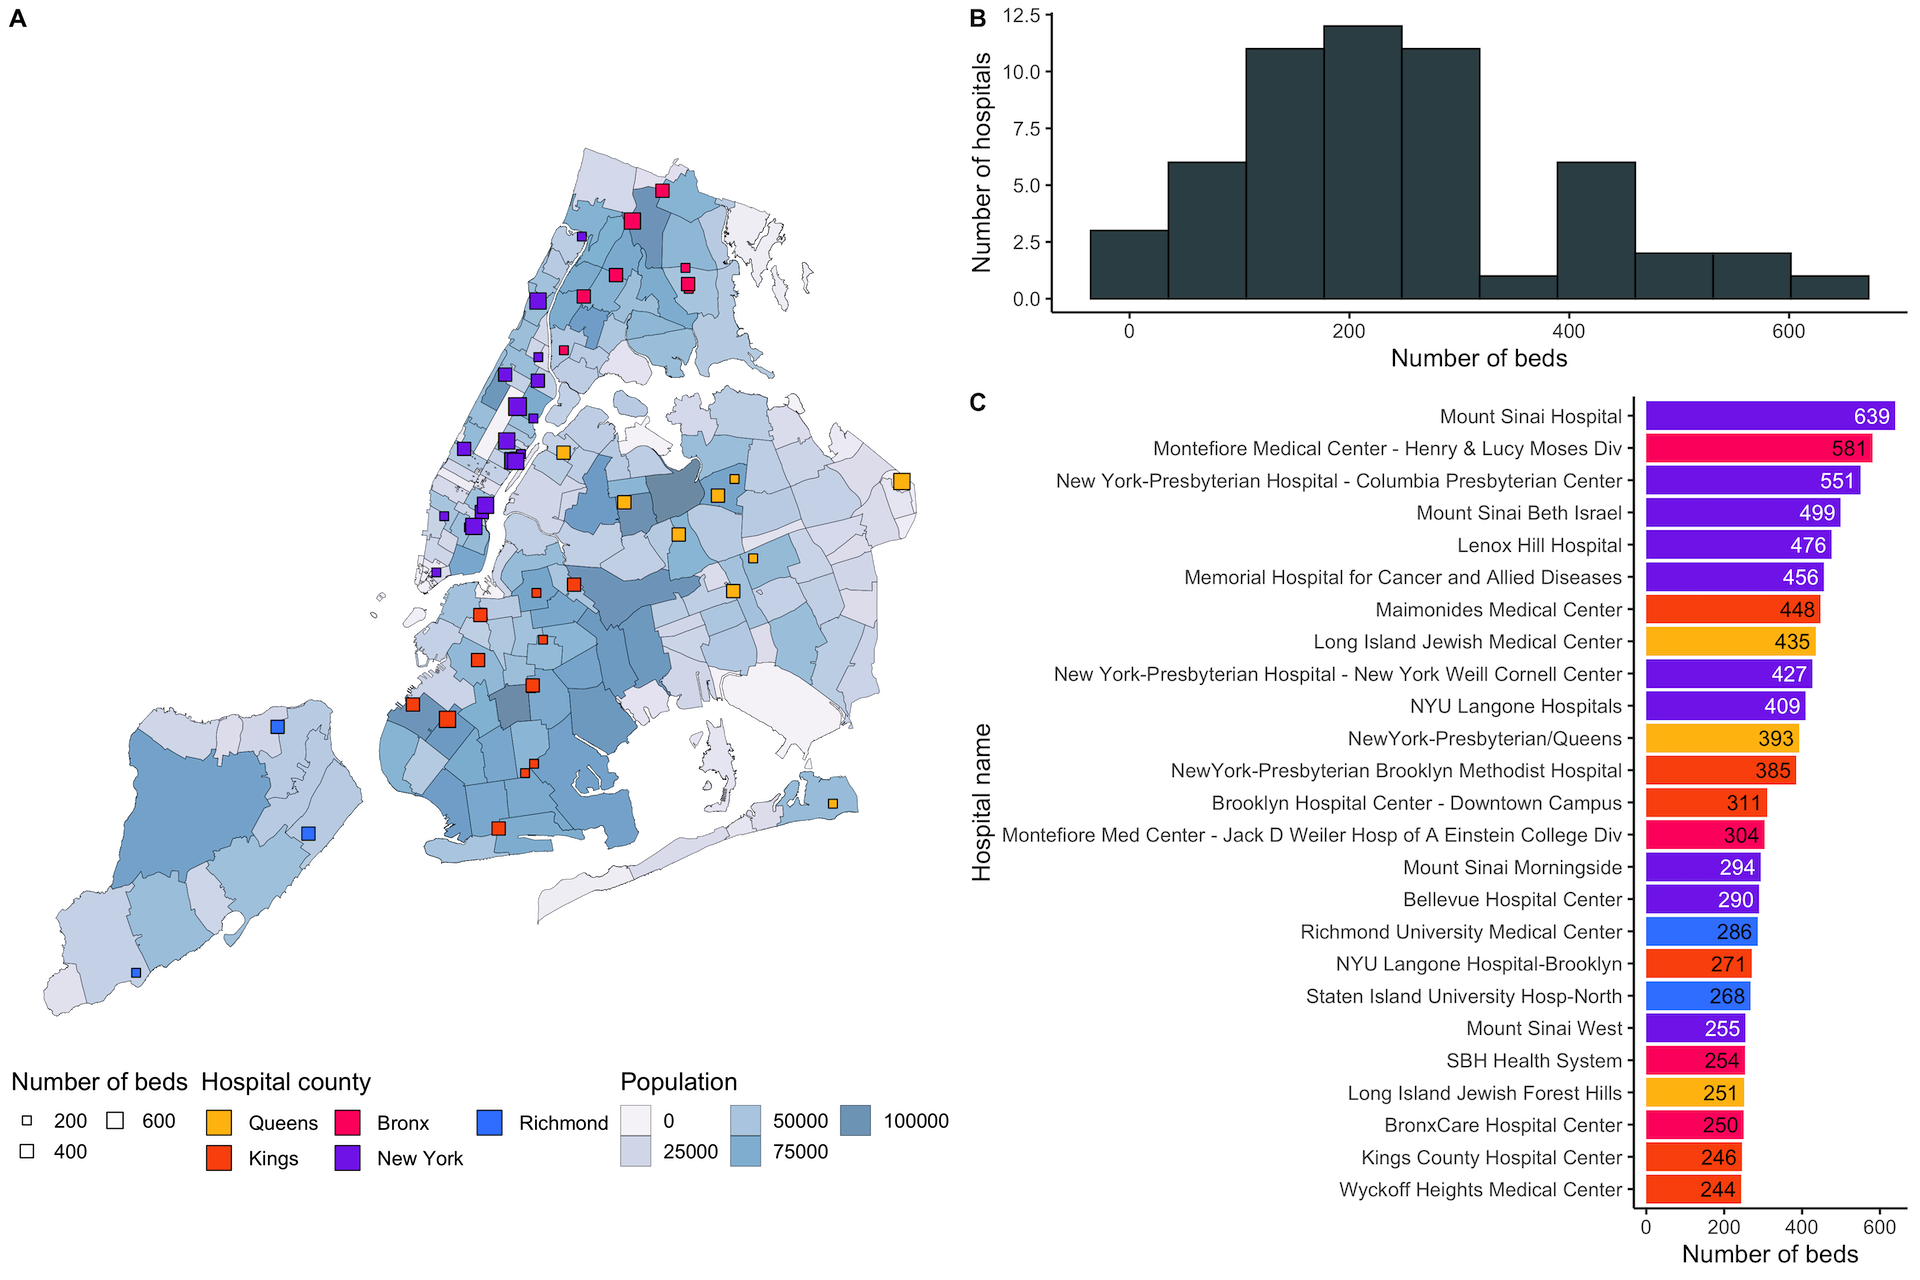
\includegraphics[width=0.9\textwidth]{images/routes/fig1.png}
    \centering
    \caption{
        \textbf{Patients routes in metropolitan France.} GPS routes with more than 5 patients are shown on map (A). Municipalities are colored by the average travel duration for patients with cancer. Patients who visit \ac{clcc} and \ac{chru} hospitals have longer travel durations (B); as well as patients who live in non-dense municipalities (C).
    }
    \label{fig:routes-duration-france}
\end{figure}

\begin{figure}[H]
    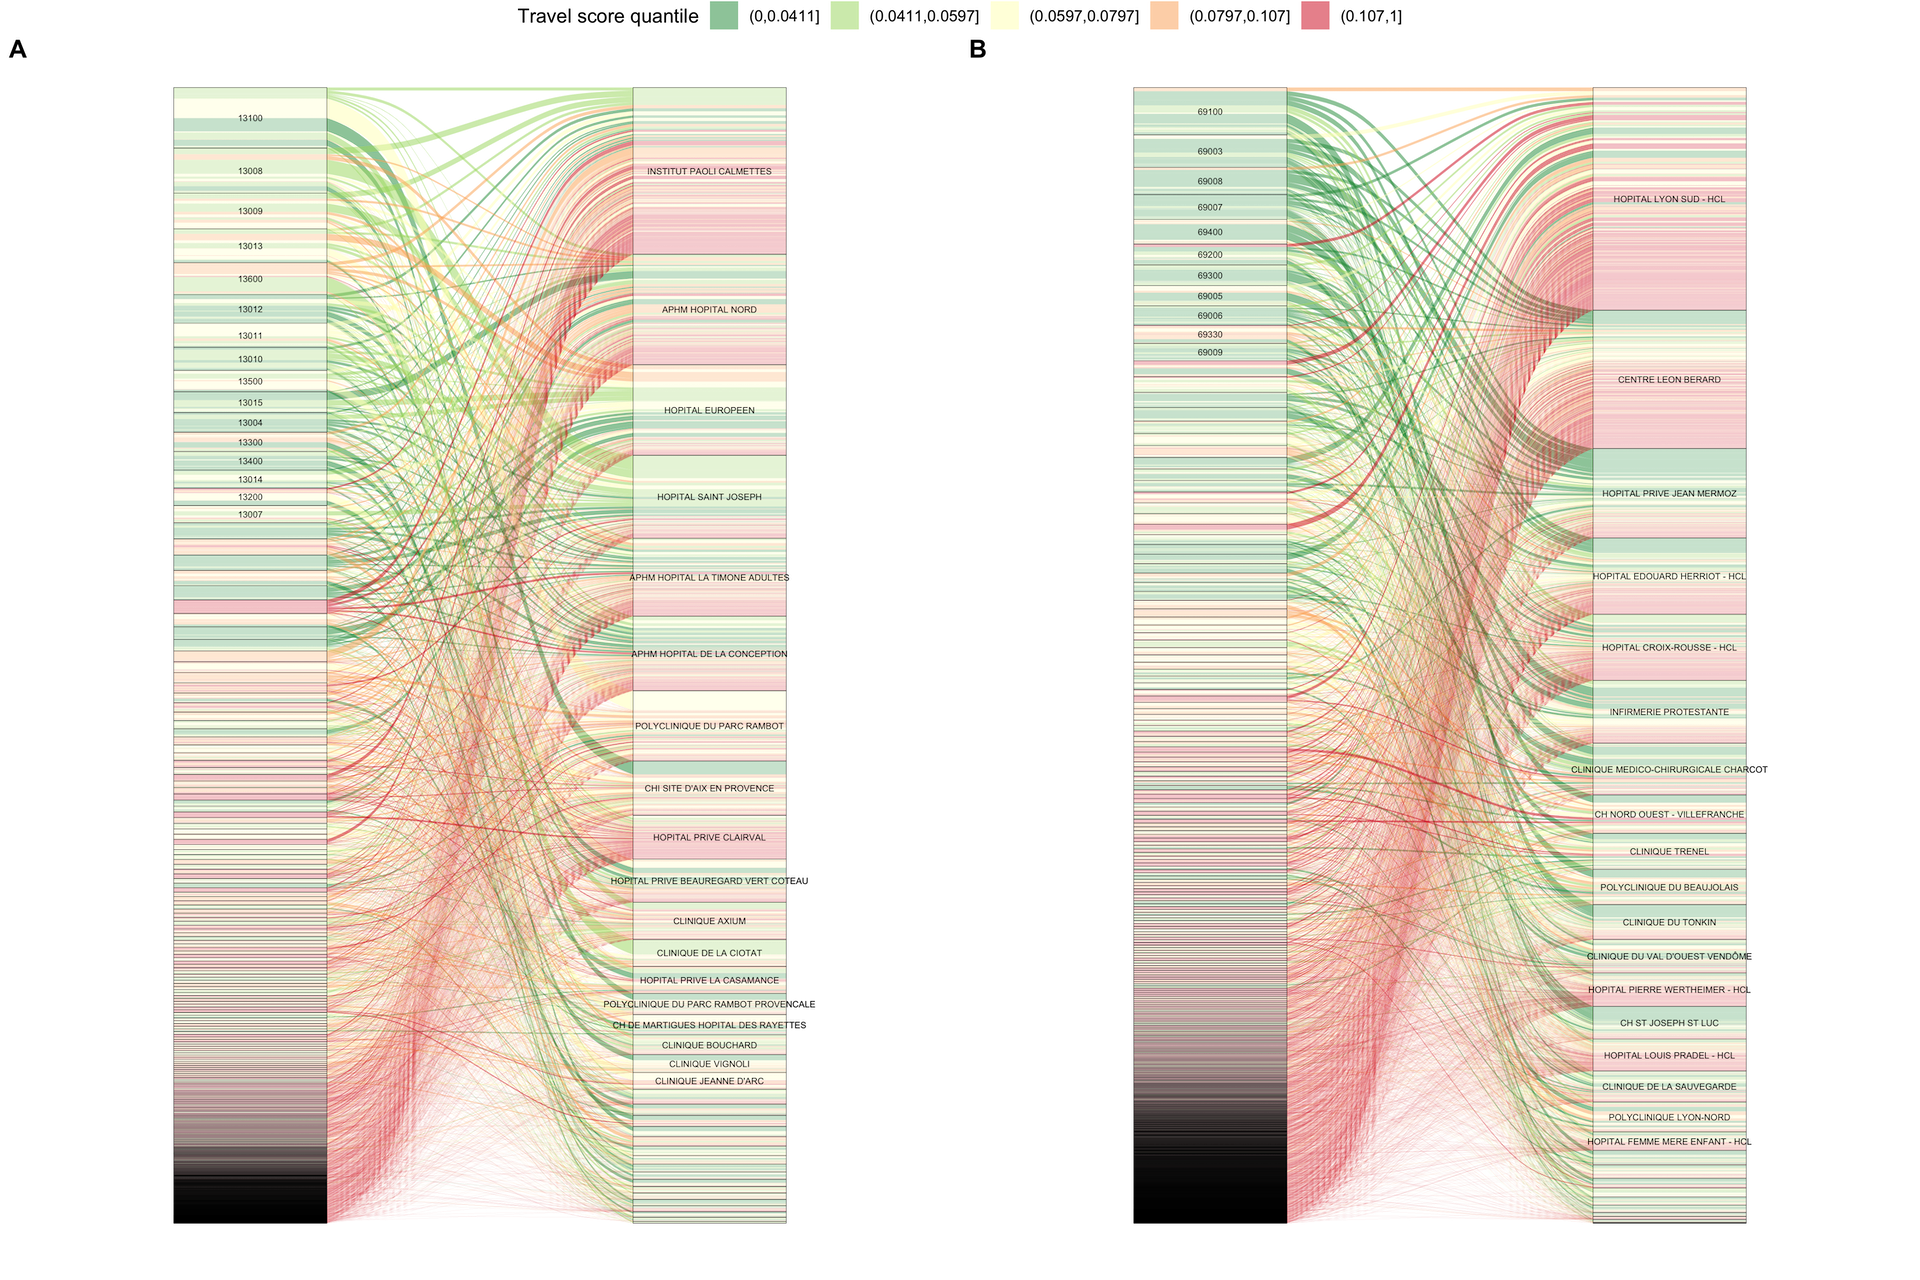
\includegraphics[width=0.9\textwidth]{images/routes/fig6.png}
    \centering
    \caption{
        \textbf{Distribution of patients traveling to care centers located in Bouches-du-Rhone department.} Municipalities are displayed on the right side of the alluvial plot, and care centers on the left side. Municipalities are sized by the number of residing patients. Care centers are sized by the number of treated patients. Flows represent patients travel and are sized by the number of patients traveling from a municipality to a care center. The flows are colored based on the travel score quantile. We can easily identify that the patients living in smaller municipalities are more likely to experience tedious travel. Larger care centers often receive patients from these smaller municipalities.
    }
    \label{fig:routes-alluvial-13}
\end{figure}

\begin{figure}[H]
    \includegraphics[width=0.9\textwidth]{images/routes/fig8.png}
    \centering
    \caption{
        \textbf{Patients travel, sized by number of travels, and colored by \ac{co2} emission.} We study the patients travel in Bourg-en-Bresse area, a sub-urban and rural area located in Auvergne-Rhone-Alpes region. Plot (A) displays the patients flows from municipalities on the right to care centers on the left. The flows are colored by the resulting \ac{co2} emissions. \ac{co2} emissions are calculated by multiplying the travel distance by the number of travels and the car average consumption. We can see that the higher \ac{co2} emissions are not issued by travels with lots of patients, but instead from travels with fewer patients but much longer drives. This is emphasized on plot (B), showing the \ac{co2} emissions resulting from patients living in Bourg en Bresse area. Indeed, the 42 travels to Hopital Lyon Sud emitted three times as much \ac{co2} than the 253 travels to Centre Hospitalier de Fleyriat.
    }
    \label{fig:routes-co2-01}
\end{figure}
